\documentclass{beamer}
\usetheme{Madrid} % My favorite!
\setbeamercovered{invisible}
% To remove the navigation symbols from 
% the bottom of slides%
\setbeamertemplate{navigation symbols}{} 
%
\usepackage{graphicx}
\usepackage{subfig}
\usepackage{caption}
\usepackage{wrapfig}

\captionsetup{figurename=,justification=justified}
\graphicspath{{figures/}}



%\usepackage{bm} % For typesetting bold math (not \mathbold)
%\logo{\includegraphics[height=0.6cm]{yourlogo.eps}}
%
\title[Anchor Placement]{Anchor Node Placement for Localization in Wireless Sensor Networks}
\author{Ben Tatham}
\institute[Carleton University]
{
Carleton University \\
Ottawa-Carleton Institute for
Electrical and Computer Engineering \\
\emph{tatham@ieee.org}
}
\date{January 19, 2011}
% \today will show current date. 
% Alternatively, you can specify a date.
%
\begin{document}
%
\begin{frame}
\titlepage
\end{frame}
%
\begin{frame}{Motivation}
\begin{block}{Why Wireless Sensor Networks?}
\begin{columns}
	\begin{column}{0.5\textwidth}
		\begin{figure}
			\centering
				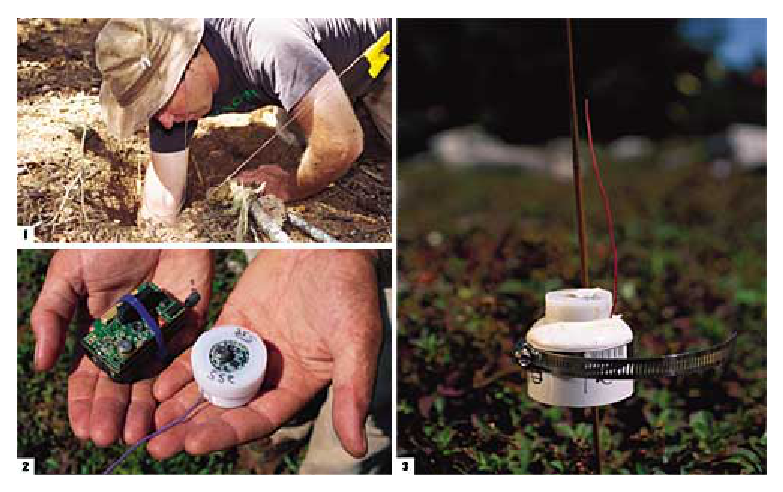
\includegraphics[width=\textwidth]{0404birdf4_123}
				\caption{Great Duck Island}
		\end{figure}
		\vfil
	\end{column}
	\begin{column}{0.5\textwidth}
		\begin{figure}
			\centering
				
\includegraphics[width=0.4\textwidth]{runes_logo}
		\end{figure}
		\vfil
	\end{column}
\end{columns}
\end{block}
\end{frame}
%
\begin{frame}{Motivation}
\begin{figure}
  \centering
    \subfloat{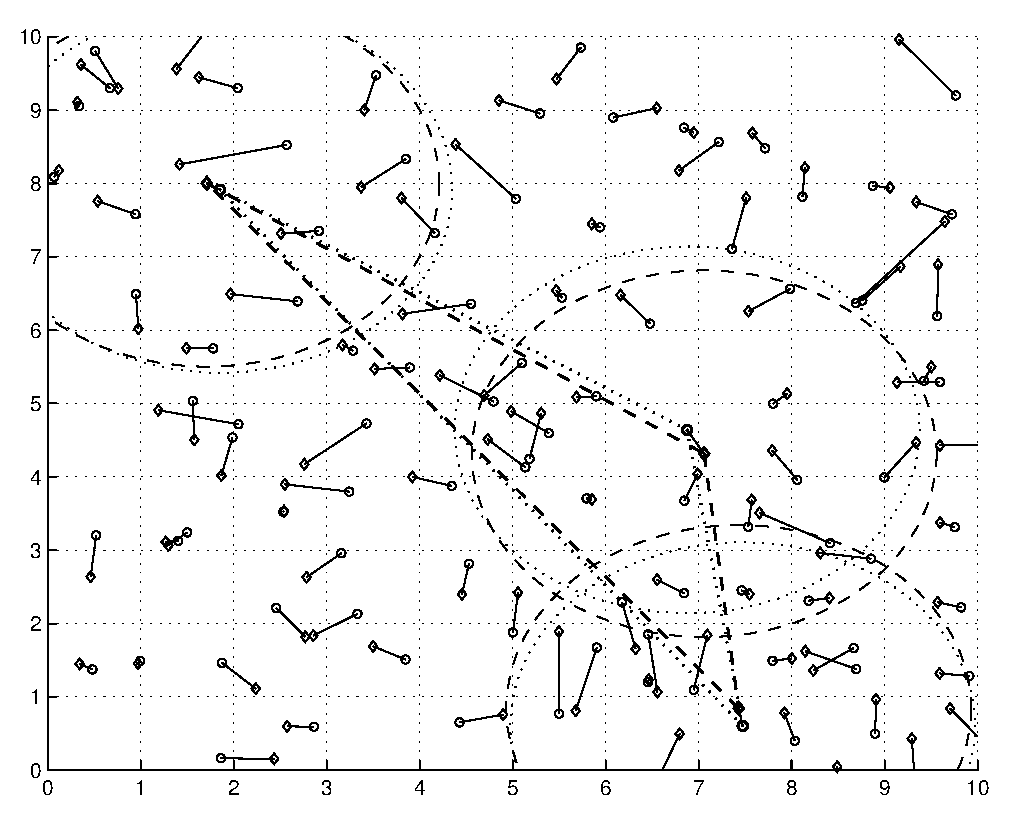
\includegraphics[width=0.32\textwidth]{motivation/plot1}}
    \subfloat{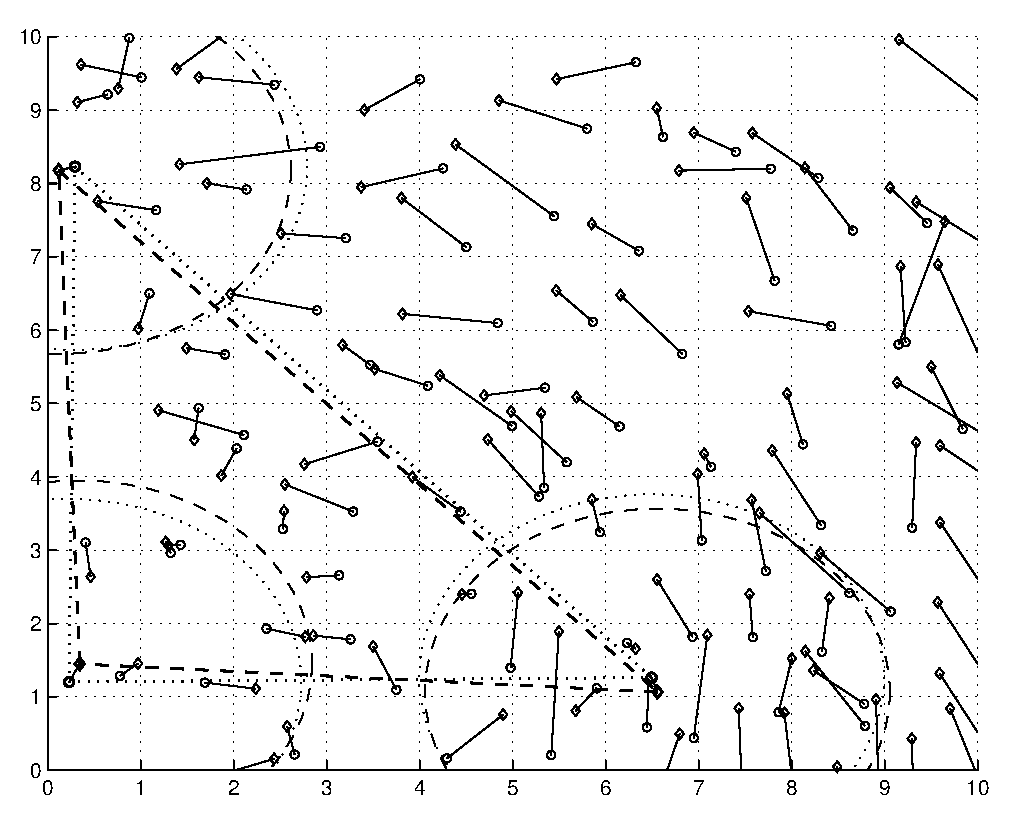
\includegraphics[width=0.32\textwidth]{motivation/plot2}}
	\\
    \subfloat{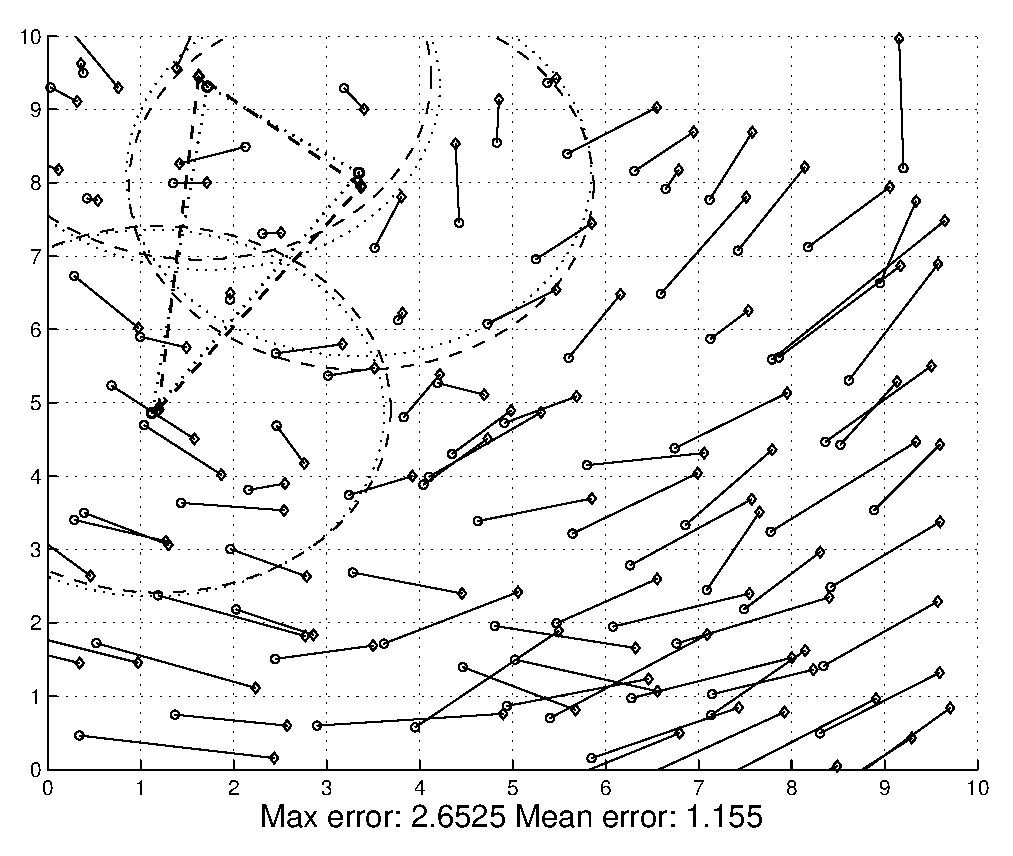
\includegraphics[width=0.32\textwidth]{motivation/plot3}}
    \subfloat{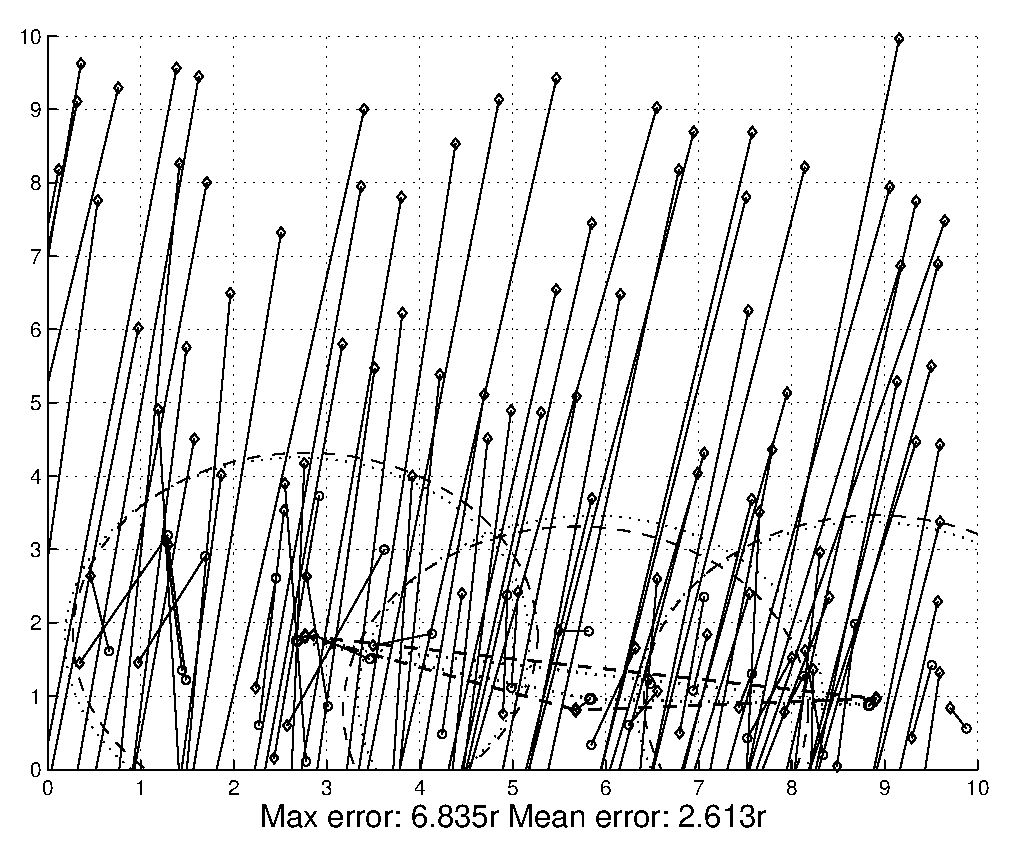
\includegraphics[width=0.32\textwidth]{motivation/plot4}}
\end{figure}
\end{frame}

\begin{frame}{The Basics}
\begin{block}{What are we actually doing?}
\begin{columns}
	\begin{column}{0.3\textwidth}
		\begin{itemize}
		\item Local to Global Coordinates
		\item Find best linear transformation
		\item $Z = b*Y*T + c$
		\end{itemize}
		\vfil
	\end{column}
	\begin{column}{0.7\textwidth}
		\begin{figure}
			\centering	
				\includegraphics[width=0.9\textwidth]{SampleAnchors}
				\caption{Procrustes Analysis}
		\end{figure}
	\end{column}
\end{columns}
\end{block}
\end{frame}

\begin{frame}{The Worst Case}
\begin{block}{What does it look like}
\begin{columns}
	\begin{column}{0.3\textwidth}
		\begin{itemize}
		\item Criss-cross effect
		\item Anchor nodes themselves are not affected
		\item Could keep points inside known region, but does not help that much
		\end{itemize}
		\vfil
	\end{column}
	\begin{column}{0.7\textwidth}
		\begin{figure}
			\centering
				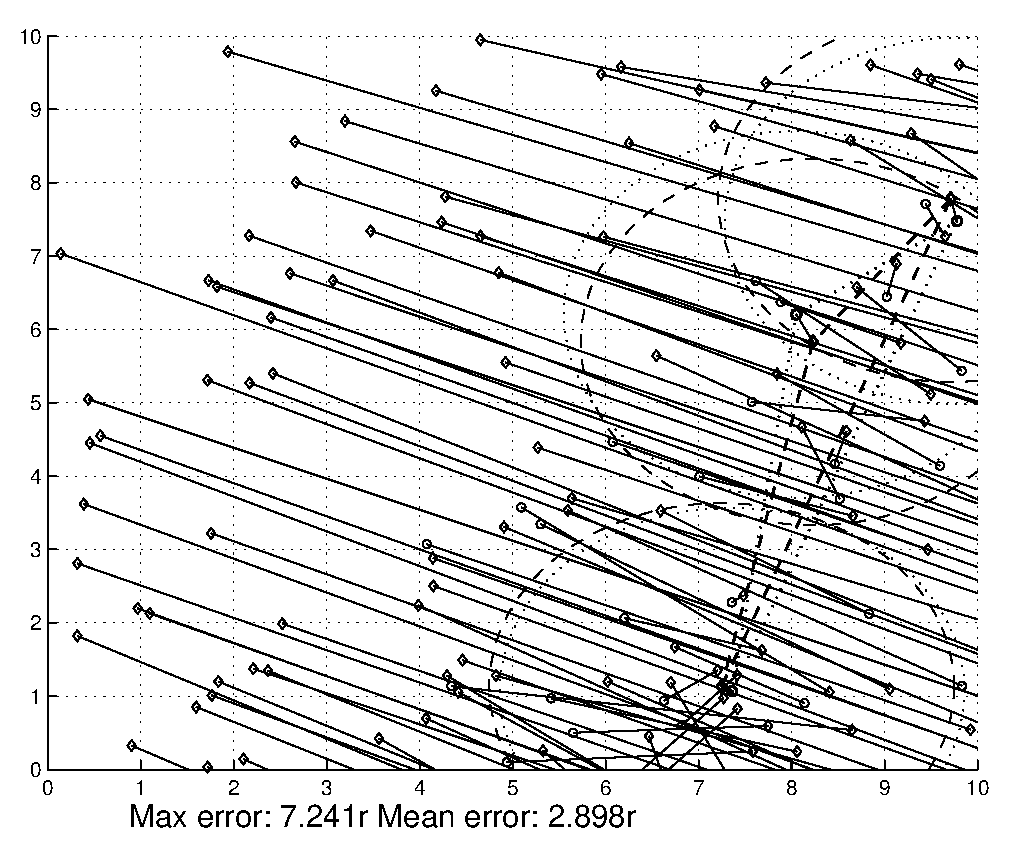
\includegraphics[width=0.7\textwidth]{AS6NetworkDiff9}
		\end{figure}
	\end{column}
\end{columns}
\end{block}
\end{frame}

\begin{frame}{The Worst Case}
\begin{block}{Avoiding it}
\begin{columns}
	\begin{column}{0.3\textwidth}
		\begin{itemize}
			\item Minimum anchor triangle heights
			\item Large height is sufficient for exclusion, but not necessary
			\item Height must be at least the radio range
		\end{itemize}
		\vfil
	\end{column}
	\begin{column}{0.7\textwidth}
		\begin{figure}
			  \centering
				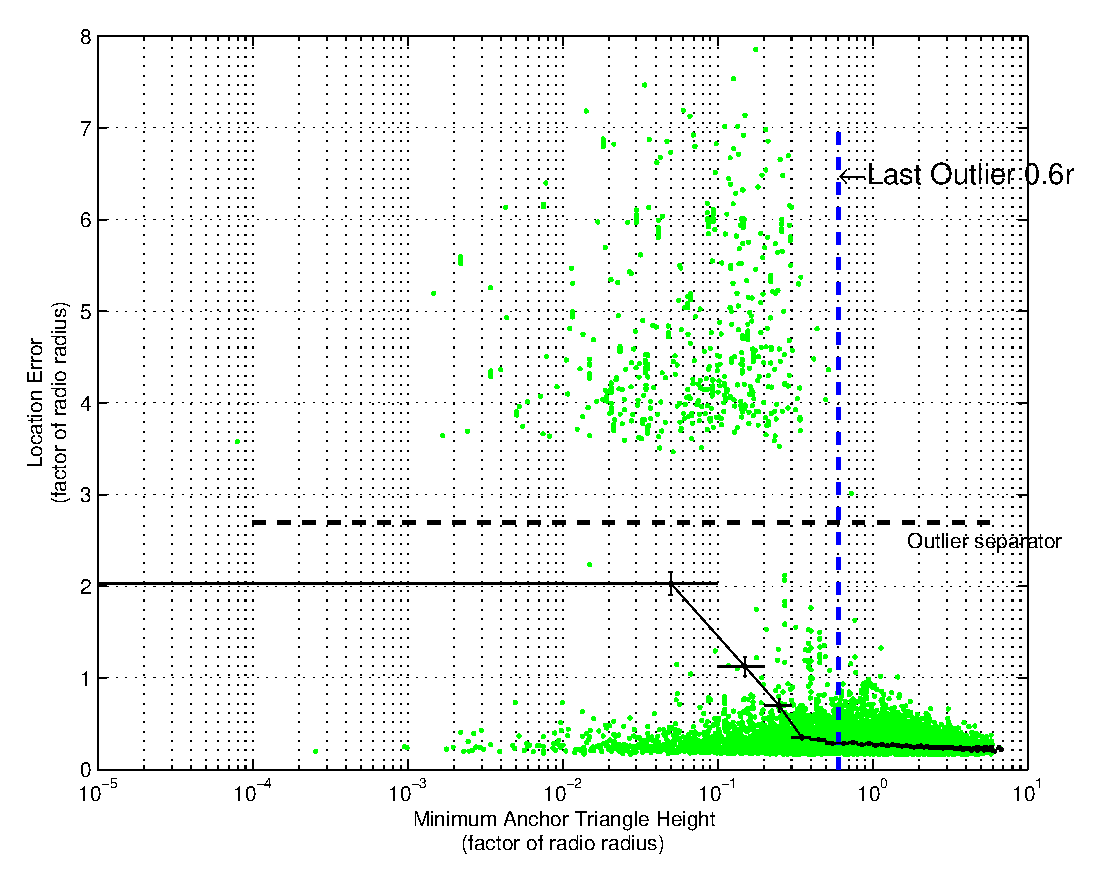
\includegraphics[width=\textwidth]{HeightIndicator_square}
				\caption{with confidence intervals grouped in intervals of 0.1r}	
		\end{figure}
	\end{column}
\end{columns}
\end{block}
\end{frame}

\begin{frame}{The Normal Case}
\begin{block}{Making the best of it}
\begin{columns}
	\begin{column}{0.3\textwidth}
		\begin{itemize}
			\item Sum of distance between anchor nodes
			\item Large height is sufficient for exclusion, but not necessary
			\item Sum must be at least 10 times the radio range
		\end{itemize}
		\vfil
	\end{column}
	\begin{column}{0.7\textwidth}
		\begin{figure}
		  \centering
			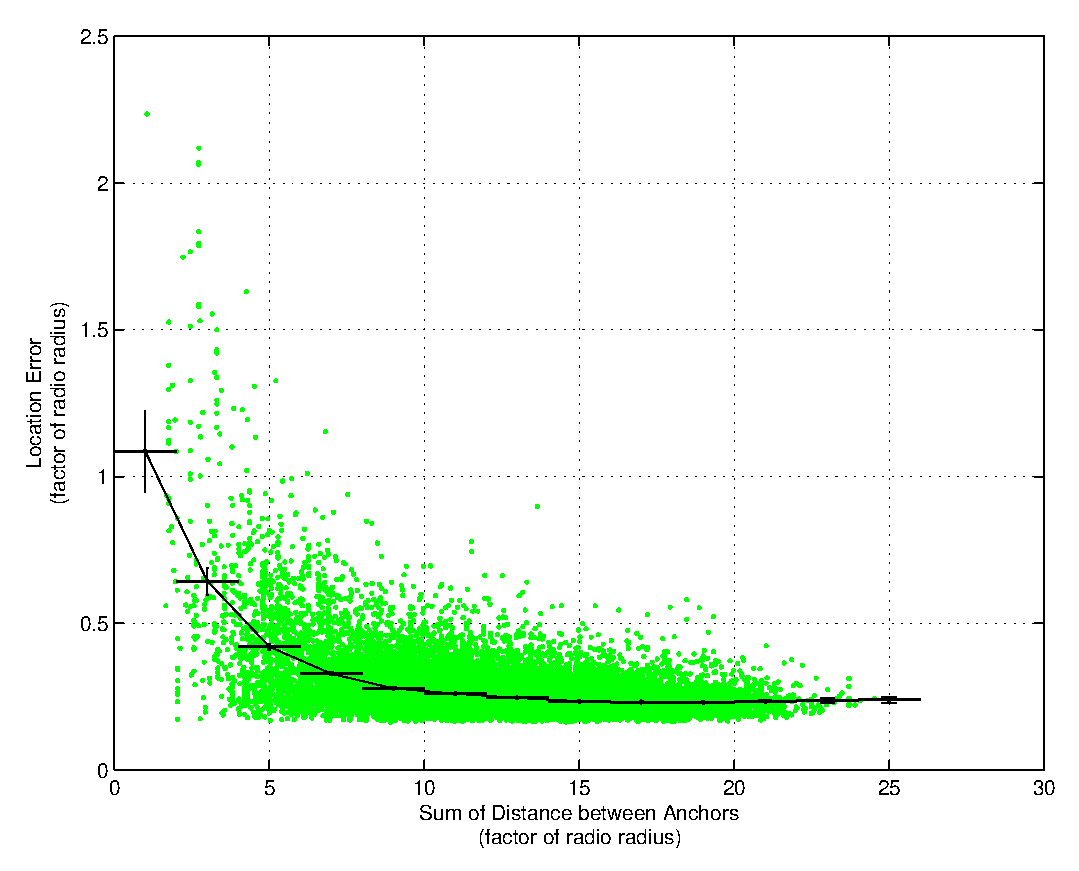
\includegraphics[width=0.7\textwidth]{SumOfDistanceIndicator_square}
			\caption{excluding outliers}
		\end{figure}
	\end{column}
\end{columns}
\end{block}
\end{frame}

\begin{frame}
\centerline{The End}
\end{frame}
% End of slides
\end{document}